\documentclass[border=10pt]{standalone}
\usepackage{tikz}
\usetikzlibrary{positioning}

% Anthropic brand colors
\definecolor{slate}{HTML}{141413}
\definecolor{ivory}{HTML}{FAF9F5}
\definecolor{clay}{HTML}{D97757}
\definecolor{sky}{HTML}{6A9BCC}
\definecolor{olive}{HTML}{788C5D}
\definecolor{gray400}{HTML}{B0AEA5}
\definecolor{gray700}{HTML}{3D3D3A}

\begin{document}
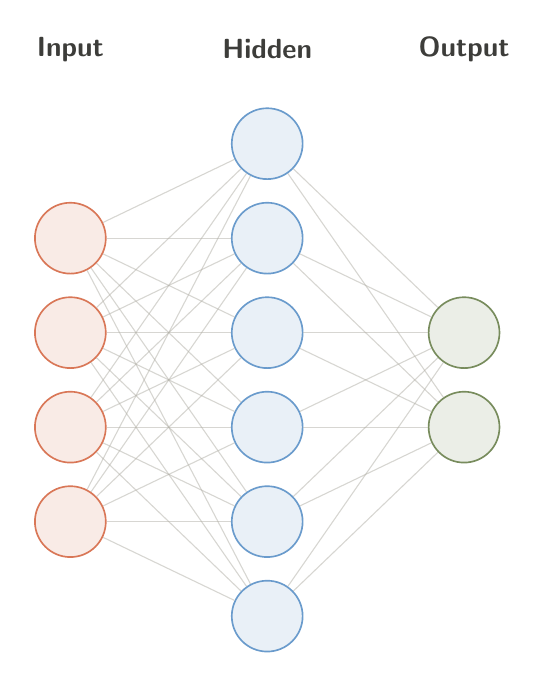
\begin{tikzpicture}[
  % Node styles
  neuron/.style={
    circle,
    draw=gray400,
    fill=ivory,
    minimum size=0.9cm,
    inner sep=0pt,
    text=slate,
    font=\sffamily\small,
    line width=0.6pt,
  },
  input neuron/.style={
    neuron,
    fill=clay!15,
    draw=clay,
  },
  hidden neuron/.style={
    neuron,
    fill=sky!15,
    draw=sky,
  },
  output neuron/.style={
    neuron,
    fill=olive!15,
    draw=olive,
  },
  % Edge style
  edge/.style={
    draw=gray400,
    line width=0.4pt,
    opacity=0.5,
  },
]

  % Spacing constants (plain numbers, in cm)
  \pgfmathsetmacro{\layersep}{2.5}   % horizontal distance between layers
  \pgfmathsetmacro{\nodesep}{1.2}    % vertical distance between nodes

  % Input layer (4 nodes) — centered at y=0
  \foreach \i in {1,...,4} {
    \pgfmathsetmacro{\ypos}{(\i - 2.5) * \nodesep}
    \node[input neuron] (I-\i) at (0, \ypos cm) {};
  }

  % Hidden layer (6 nodes) — centered at y=0
  \foreach \i in {1,...,6} {
    \pgfmathsetmacro{\ypos}{(\i - 3.5) * \nodesep}
    \node[hidden neuron] (H-\i) at (\layersep cm, \ypos cm) {};
  }

  % Output layer (2 nodes) — centered at y=0
  \foreach \i in {1,...,2} {
    \pgfmathsetmacro{\ypos}{(\i - 1.5) * \nodesep}
    \node[output neuron] (O-\i) at (2*\layersep cm, \ypos cm) {};
  }

  % Edges: input -> hidden
  \foreach \i in {1,...,4} {
    \foreach \j in {1,...,6} {
      \draw[edge] (I-\i) -- (H-\j);
    }
  }

  % Edges: hidden -> output
  \foreach \i in {1,...,6} {
    \foreach \j in {1,...,2} {
      \draw[edge] (H-\i) -- (O-\j);
    }
  }

  % Layer labels — all at the same y-coordinate (above tallest layer + margin)
  \pgfmathsetmacro{\labelY}{(6 - 1) / 2 * \nodesep + 1.2}  % top of hidden layer + margin
  \node[font=\sffamily\bfseries, text=gray700] at (0, \labelY cm) {Input};
  \node[font=\sffamily\bfseries, text=gray700] at (\layersep cm, \labelY cm) {Hidden};
  \node[font=\sffamily\bfseries, text=gray700] at (2*\layersep cm, \labelY cm) {Output};

\end{tikzpicture}
\end{document}
